\begin{frame}{Construction of conservative nodal normals}
  \begin{gather*}
    \bm n^i = \int_\Gamma \phi^i \bm n
  \end{gather*}
  \begin{itemize}
  \item Exact conservation even with rough surfaces
  \item Definition is robust in 2D and for first-order elements in 3D
  \item $\int_\Gamma \phi^i = 0$ for corner basis function of undeformed $P_2$ triangle
  \item May be negative for sufficiently deformed quadrilaterals
  \item Mesh motion should use normals from CAD model
    \begin{itemize}
    \item Difference between CAD normal and conservative normal introduces correction term to conserve mass within the mesh
\item Anomolous velocities if disagreement is large \\ (fast moving mesh, rough surface)
    \end{itemize}
  \item Normal field not as smooth/accurate as desirable \\ (and achievable with non-conservative normals)
    \begin{itemize}
    \item Mostly problematic for surface tension
    \item Walkley et al, \emph{On calculation of normals in free-surface flow problems}, 2004
    \end{itemize}
  \end{itemize}
\end{frame}

\begin{frame}{Need for well-balancing}
  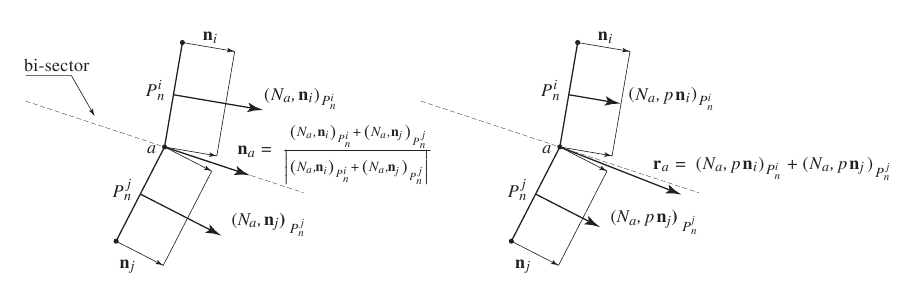
\includegraphics[width=\textwidth]{figures/slip/Behr2004-NormalVsResidual} \\
  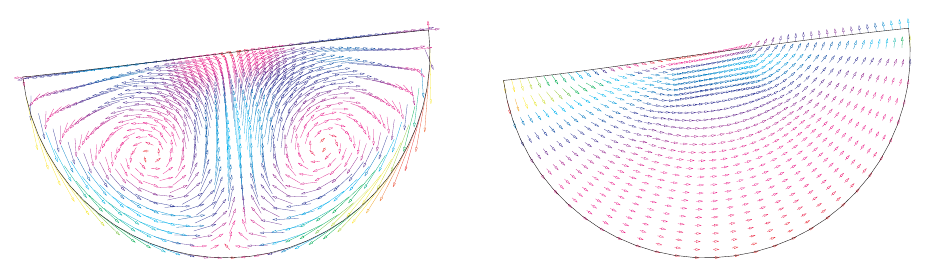
\includegraphics[width=\textwidth]{figures/slip/Behr2004-NavierSloshing} \\
  \footnotesize{(Behr, \emph{On the application of slip boundary condition on curved surfaces}, 2004)}
\end{frame}

\begin{frame}{``No'' boundary condition}
  \begin{itemize}
  \item Integration by parts produces
    \begin{gather*}
      \int_\Gamma \bm v \cdot T \bm\sigma \cdot \bm n, \qquad \bm\sigma = \eta D \bm u - p\bm 1, \qquad T = \bm 1 - \bm n \otimes \bm n
    \end{gather*}
  \item Continuous weak form requires either
    \begin{itemize}
    \item Dirichlet: $\bm u |_{\Gamma} = \bm f \implies \bm v|_\Gamma = 0$
    \item Neumann/Robin: $\bm\sigma\cdot\bm n |_\Gamma = \bm g(\bm u,p)$
    \end{itemize}
  \item Discrete problem allows integration of $\bm\sigma\cdot\bm n$ ``as is''
    \begin{itemize}
    \item Extends validity of equations to include $\Gamma$
    \item \alert{Not valid} for continuum equations
    \item Introduced by Papanastasiou, Malamataris, and Ellwood, 1992 for Navier-Stokes outflow boundaries
    \item Griffiths, {\small \emph{The `no boundary condition' outflow boundary condition}, 1997}
      \begin{itemize}
      \item Proves $L^\infty$ order of accuracy $\bigO((h + 1/\Peclet)^{p+1})$ \\
        for Galerkin finite elements of order $p$ (linear advection-diffusion)
      \item Demonstrates equivalence with collocation at Radau points \\ in outflow element
      \end{itemize}
    \item Used in slip boundary conditions by Behr 2004
    \end{itemize}
  \end{itemize}
\end{frame}
